\begin{frame}[parent={cmap:software-testing},hasnext=true,hasprev=true]
\label{concept:test-criterion}
\frametitle{Test criterion}

\begin{block:concept}{Definition}
A test criterion systematizes the way test requirements are
generated from the source of information (specification, source code,
historical fault database, etc.).
\end{block:concept}

\begin{block:fact}{}
\begin{itemize}
	\item A test criterion provides a systematic way to select test cases.
	\begin{itemize}
		\item A testing criterion divides the input domain.
	\end{itemize}

	\item When no faults are found, test criterion provides an indication of
	how test cases should be selected in order to establish a high level of
	confidence of product correction.
\end{itemize}
\end{block:fact}

\hfill
\refie{example:test-criterion}{\beamerbutton{Example: Test criterion example}}
\end{frame}


\begin{frame}
\frametitle{Test criterion}

\begin{block:fact}{Test criterion attributes}
\begin{itemize}
	\item A test criterion can be compared based on cost, efficacy and
	strength.
\end{itemize}
\end{block:fact}

\begin{figure}
    \centering
    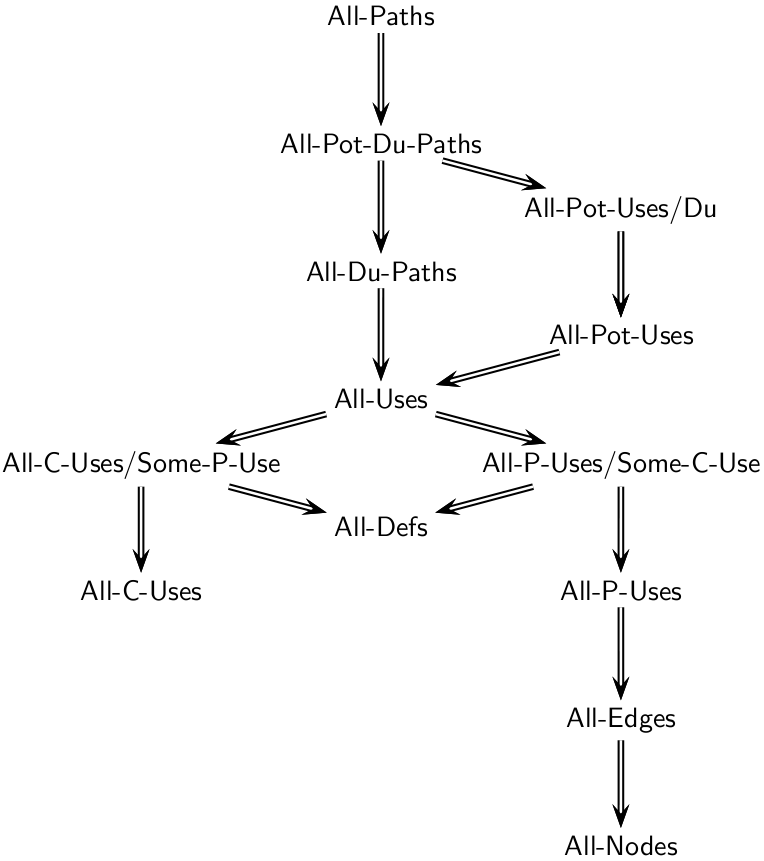
\includegraphics[width=4cm]{subsume-relation}
\end{figure}
\end{frame}
